\documentclass{sig-alternate}

\usepackage{listings}
\usepackage{hyperref}

% Custom colors
\usepackage{color}
\definecolor{deepblue}{rgb}{0,0,0.5}
\definecolor{deepred}{rgb}{0.6,0,0}
\definecolor{deepgreen}{rgb}{0,0.5,0}

\begin{document}
%
% --- Author Metadata here ---
\conferenceinfo{Blocks and Beyond}{'15 Atlanta, Georgia USA}
%\CopyrightYear{2007} % Allows default copyright year (20XX) to be over-ridden - IF NEED BE.
%\crdata{0-12345-67-8/90/01}  % Allows default copyright data (0-89791-88-6/97/05) to be over-ridden - IF NEED BE.
% --- End of Author Metadata ---
% From Interest to Usefulness
\title{BlockPy: From Interest to Usefulness in a Block-based Environment}
\numberofauthors{1}
\author{
	\alignauthor {Austin Cory Bart, Eli Tilevich, Clifford A. Shaffer, Dennis Kafura}\\
	\email{\{acbart, tilevich, shaffer, kafura\}@vt.edu}\\
	\affaddr{Virginia Tech}  \\
}
\date{30 July 1999}

\maketitle
\begin{abstract}
As block-based environments are used for more mature audiences, the environments must mature themselves.
Based on holistic theories of academic motivation, this means making the environment present itself as both Interesting \textit{and} Useful, without sacricing pedagogical power and scaffolding.
We present Data Science as a potential context that satisfies all of these constraints, and describe our new Blockly-based programming environment that supports Data Science from day one: \url{http://think.cs.vt.edu/blockpy/}.
Our new open-source tool BlockPy features a number of other powerful features meant to suggest authenticity and promote transfer for students as they mature.
This includes Mutual Language Translation and inline code embedding, but also powerful tools for getting real-world data and visualizing it.
As we have developed the tool, we have identified a number of major research questions that should be answered in order to determine the validity of our hypothesis and the potential of our approach.
\end{abstract}

% A category with the (minimum) three required fields
\category{K.3.2}{Computer and Information Science Education}{Computer Science Education}

\terms{Design, Human Factors, Reliability, Experimentation}

\keywords{Blockly, Kennel, Interest, Usefulness} % NOT required for Proceedings


\section{Introduction}

Many universities are now defining core credit hours in subjects such as ``Computational Thinking'', subsets of Computer Science knowledge meant for solving interdisciplinary problems using some degree of programming.
This means that universities now have students of every different discipline and background taking a programming course.
There are implications for this different class of learners that are still becoming apparent to education researchers, beyond issues related to students' aptitude.
Students with a clearly domain-identified interest (i.e. their actual major) can view introductory computing courses with doubt and suspicion -- what does this course have to offer them?
Since they do not have much time to spare, they might deprioritize a ``fun'' classes homework over a ``useful'' classes.

Our position is that, in order to fully engage mature cross-university undergraduate students, an introductory programming environment should be both interesting \textit{and} useful.
Critically, this means that the environment should enable working with a context that students relate to, find enjoyable, and helps them solve useful problems.
Furthermore, they should feel that the material that they're learning will help them to transition to more authentic, serious problem-solving, such as that mediated by traditional, text-based, mature programming environments.
These changes should not come at the cost of the scaffolding that makes these environments pedagogical valuable, but instead should provide new opportunities for students' learning.

Block-based environments like Scratch and Snap! have already been successful with younger students, particularly in high-school settings.
In addition to side-stepping syntax headaches, these environments make it easier to get working with the motivating educational context, such as game and animation design, robots, or media computation, because they immediately expose the range of actions afforded by the context (e.g., a ``draw a circle'' block for media computation) and support the experiences at a high level (e.g., a drawing canvas embedded within the environment).
These contexts can be very popular with certain classes of students: young male children usually enjoy creating games, for example, so game and animation design is a very compelling hook.
However, block-based languages are now expanding into the university level, with a more diverse population that may view them as a toy rather than a useful tool -- simply because of the existing contexts that they are providing.

We submit \textit{Data Science} as a context that block-based environments should support as a first-class citizen, similar to how Snap! and Scratch support game design.
Data Science for Introductory Computing is a growing movement, with many instructors recognizing the inherent value ~\cite{Anderson, Sullivan:2013}
Data science provides an authentic, useful context for every kind of students, since exploring data-oriented problems is something that almost all fields are beginning to find relevant~\cite{Layman:2007, Social-good}.
Additionally, it is readily possible to find data sources that connect to the world around the student and their past experiences, establishing a sense of personalized interest.
When students inevitably ask, ``What am I going to be using this for?'', it is possible to point to well-defined data problems in their field requiring computation.

\begin{figure*}[t]
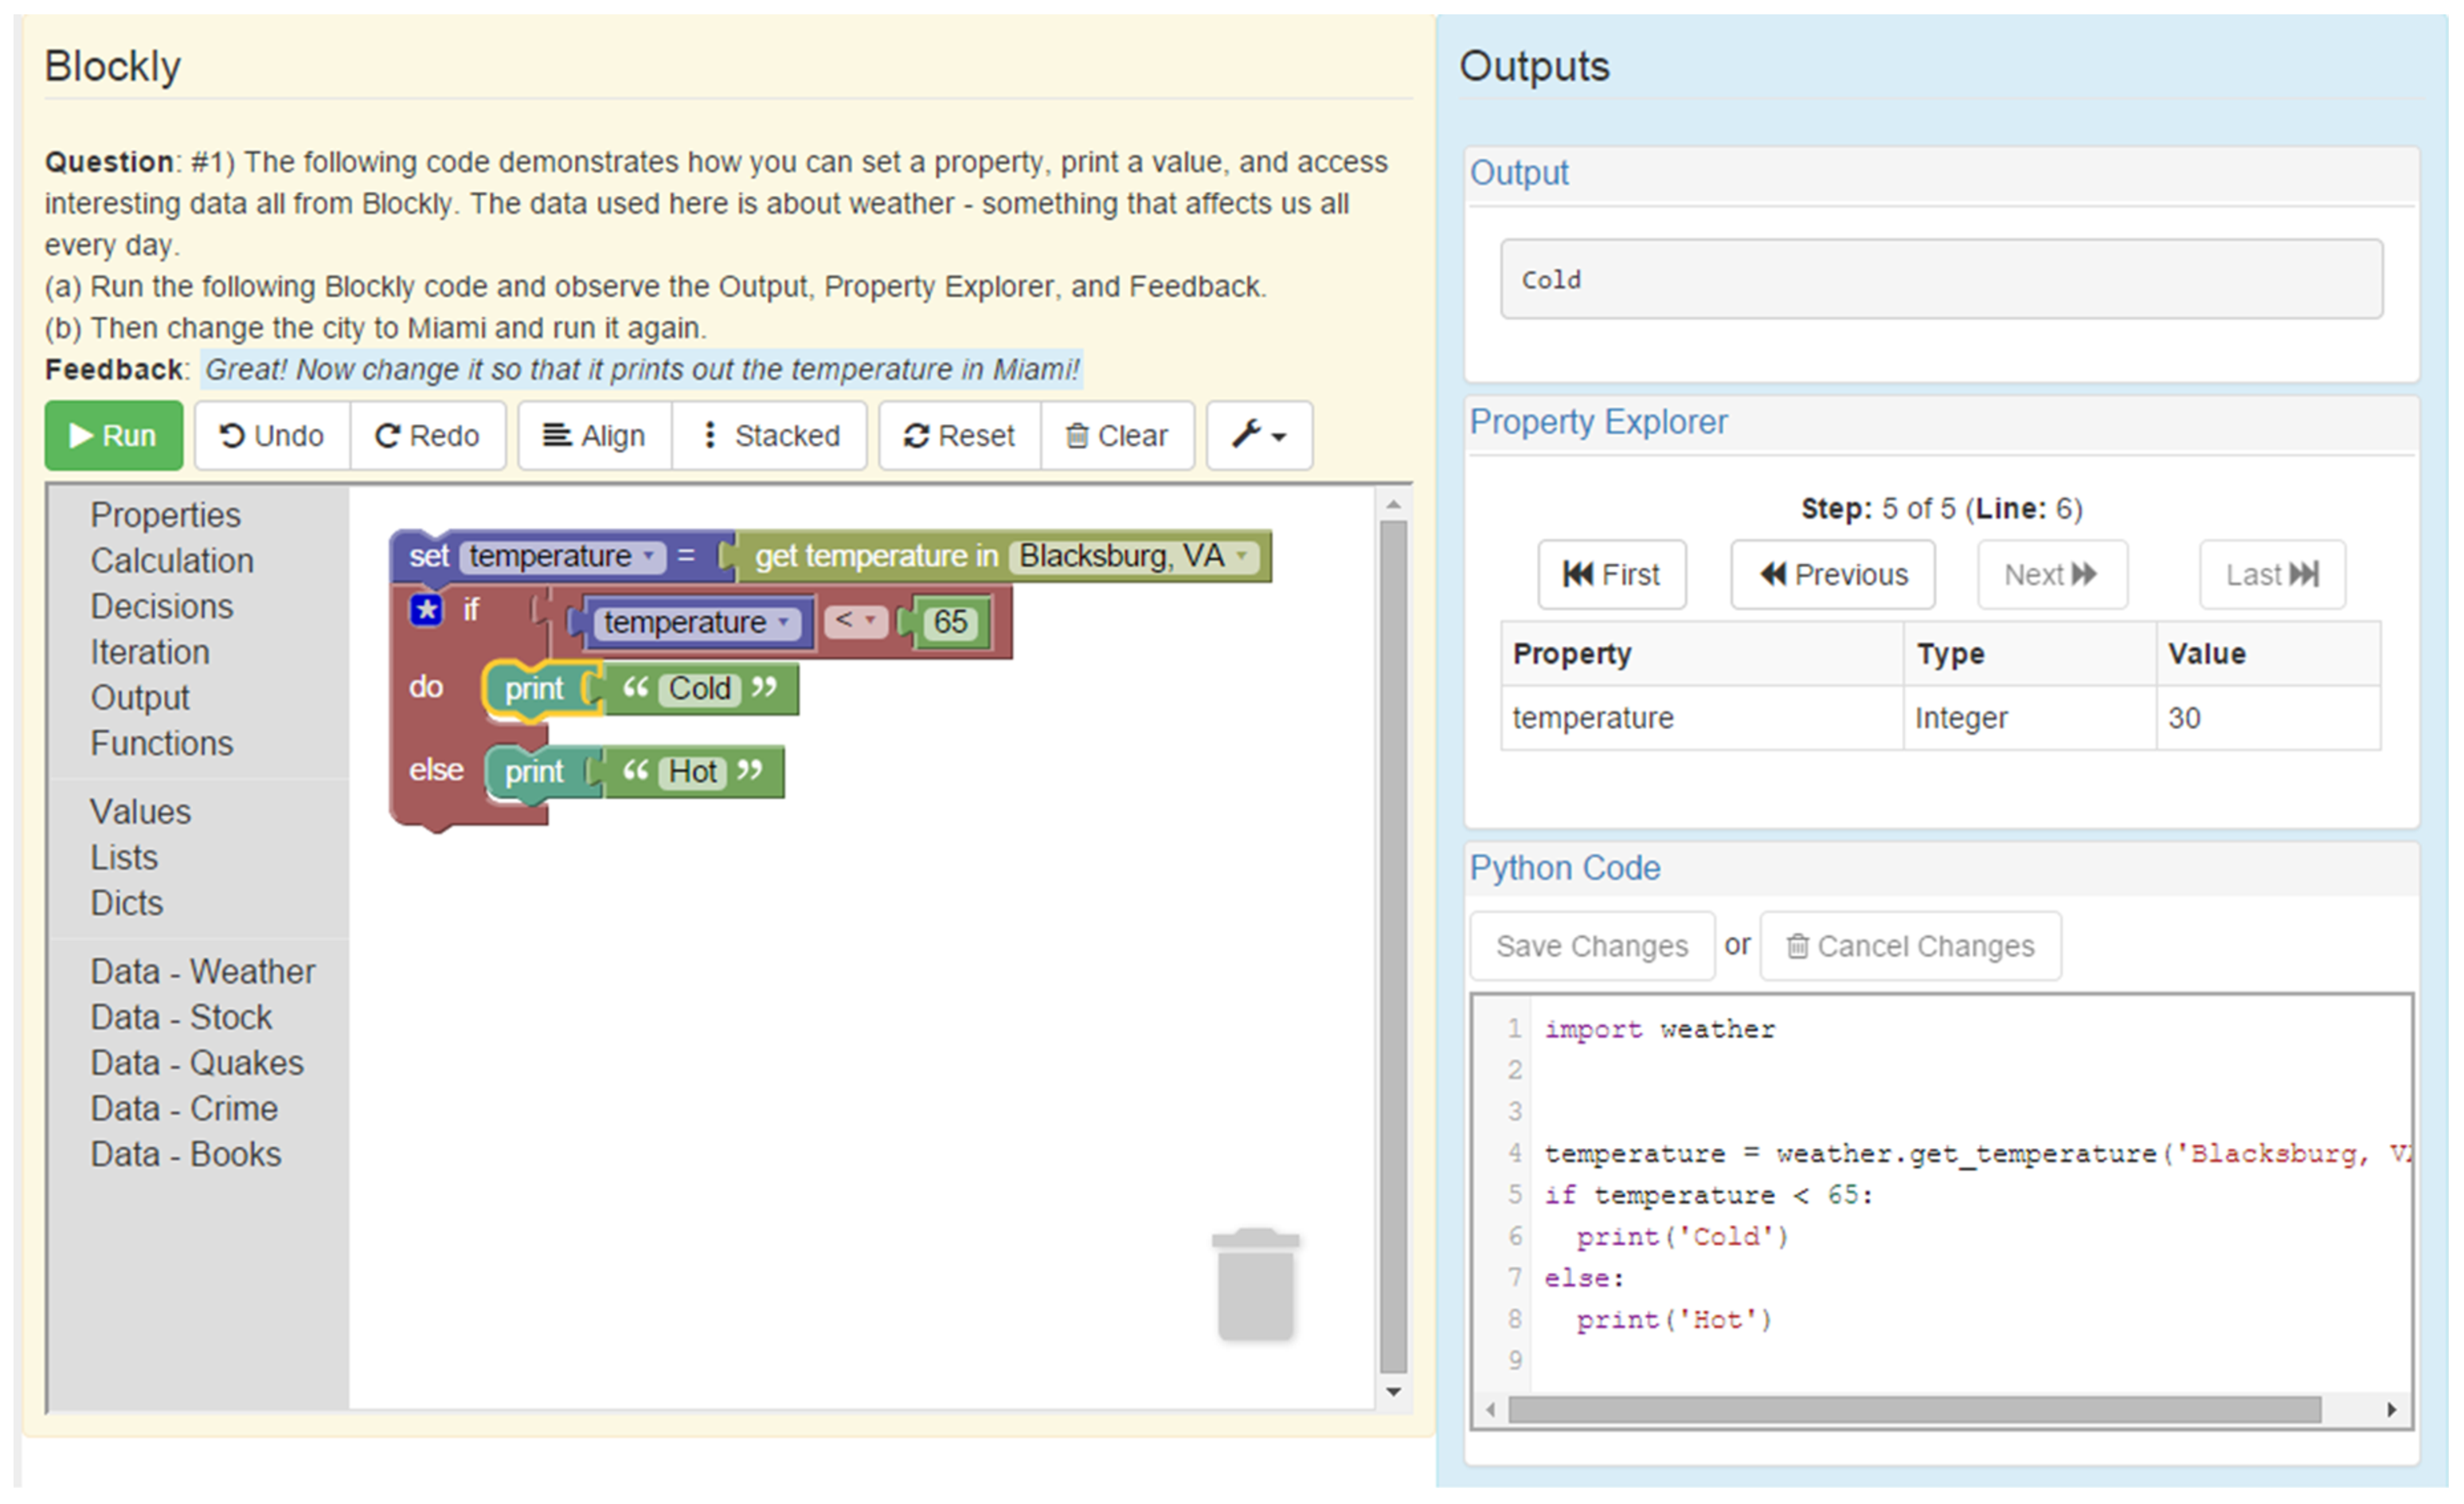
\psfig{file=images/full-kennel.eps, width=\linewidth}
\caption{A complete representation of BlockPy}
\label{fig-blockpy-full}
\end{figure*}

\subsection{Academic Motivation and Blocks}

Understanding the motivational construct of ``Interest'' is a complicated problem. The MUSIC model of academic motivation\cite{jones-description} differentiates between five different components of motivation, explicitly drawing a line between them: \textbf{eMpowerment}, the amount of control that a student feels that they have over their learning experience; \textbf{Usefulness}, the expectation of the student that the material they are learning will be valuable to their short-term and long-term goals; \textbf{Success}, the student's belief in their own ability to complete their work; \textbf{Interest}, the student's perception of how the assignment appeals to situational or dispositional interests; and \textbf{Caring}, the students perception of their professor's and classmates attitudes toward them.
A student becomes motivated when they perceive one or more of these constructs in their learning experience.
Students individually differ in what they want and need when it comes to motivation, and there are few one-size-fits-all solutions.
An instructor needs to plan across each of these dimensions to cover as many bases as possible, and therefore the environment should support this process.

There have been a few empirical studies looking at the effect of Block-based programming environments on motivation in undergraduate introductory computing.
Mishra~\cite{Mishra} conducted a two-week intervention in a a CS-1 course where students worked with Scratch before they began working with Java, reporting positive outcomes in both learning and engagement.
However, although the sample population was quite large (N=450), the students do not represent the typical body of a university: they were non-CS engineering majors, 88\% male, and ``highest ranked'' in ``mathematics, physics, and chemistry''.
The students did vary greatly on prior programming performance, but it is likely that they have rather uniform motivational concerns, compared to a more diverse student body.
The perception survey revealed that many students cited the game design context afforded by Scratch as a major motivating factor: ``[I am] thrilled to be able to code complex games'' and ``[coding] games helped increase my interest, [...], there was lot of room for experimentation.''
Further research is required to determine if more diverse populations have different perceptions of the environments' motivational value -- to that end, we have created a new block-based environment to appeal to a different facet of motivation.

\section{BlockPy}
	
In this section, we outline our work on a new block-based environment, a beginner-friendly programming environment that scaffolds the learner into a more mature environment while supporting a sense of Usefulness up-front.
The tool is online now at \url{http://think.cs.vt.edu/blockpy/} and open-sourced on GitHub.
Internally, Kennel uses a modified version of the open-source Blockly library to provide a block editor, a modified version of the open-source Skulpt library to execute Python code client-side, and an unmodified version of the open-source CodeMirror library to provide a text editor.
Students can, from day one, start using data science features built-in to the system to work on guided practice problems.
The system promotes the learning transfer process by supporting Mutual Language Transformation between Blockly and Python -- at any time, code can be viewed in the block editor and the text editor.
Additionally, Python expressions and code blocks can be inlined inside of a Blockly program in order to support partial transitions.

\subsection{Data Science as a First-Class Feature}

%\begin{figure*}[ht]
%\centering
%\begin{minipage}[b]{0.45\linewidth}
%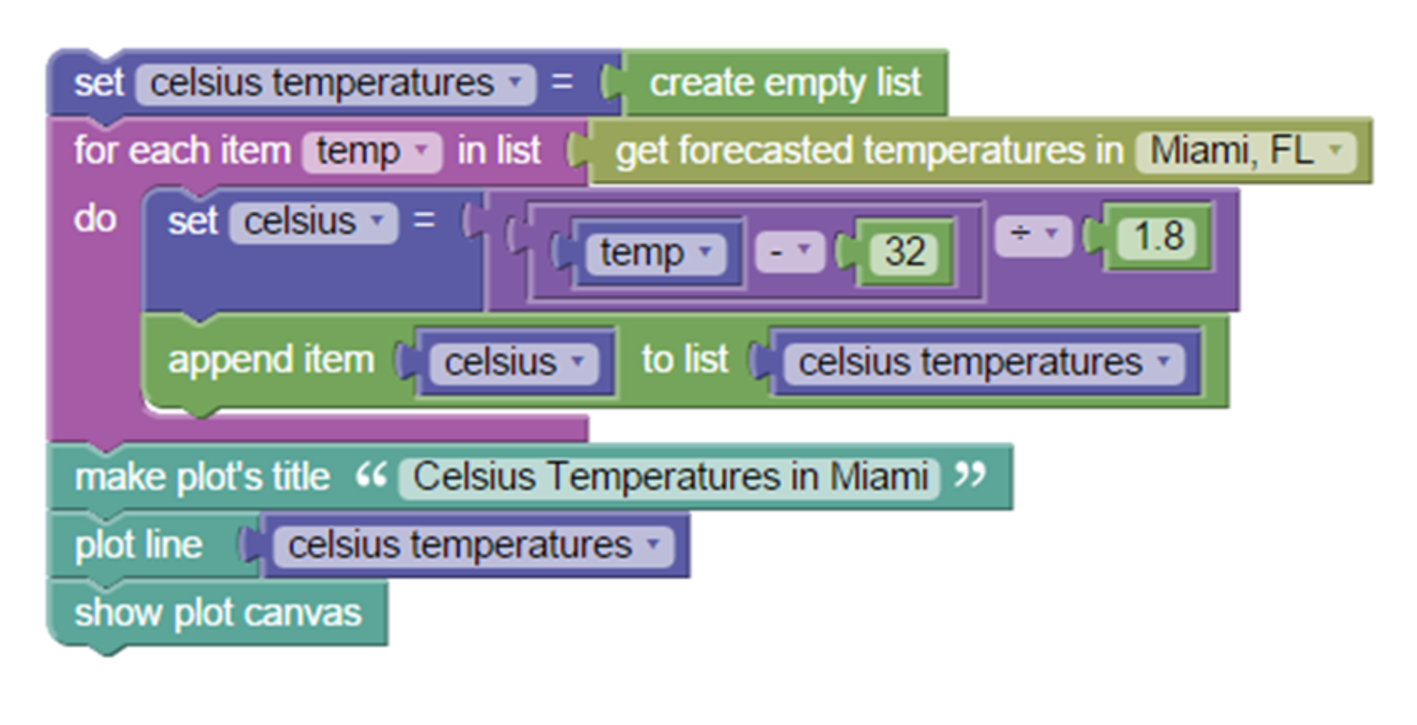
\psfig{file=images/blockly-example.eps, width=\linewidth}
%\end{minipage}
%\quad
%\begin{minipage}[b]{0.45\linewidth}
%\definecolor{mymauve}{rgb}{0.58,0,0.82}
%\lstset{stringstyle=\color{mymauve}}
%\begin{lstlisting}[language=Python, 
%showstringspaces=false,
%basicstyle=\ttfamily,
%columns=flexible,
%keepspaces=true,
%otherkeywords={import, for, in, as},
%keywordstyle=\ttfamily\color{deepblue},
%]
%import weather
%import matplotlib.pyplot as plt
%
%celsius_temperatures = []
%for t in weather.get_temperatures('Miami, FL'):
  %celsius = (t - 32) / 1.8
  %celsius_temperatures.append(celsius)
%plt.title('Celsius Temperatures of Miami')
%plt.plot(celsius_temperatures)
%plt.show()
%\end{lstlisting}
%\end{minipage}
%\caption{Mutual Language Translation is used to automatically support bi-directional translation between the blocks view and text view}
%\label{fig-mlt}
%\end{figure*}

This system includes a number of first-class features for Data Science, many adapted from professional programming environments.
Special APIs and blocks have been added that make it trivial to integrate real-time data sources such as weather information, earthquake reports, and stock feeds, as demonstrated by figure \ref{fig-blockpy-full}.
Data returned from their interface is extremely simple -- usually either primitive (numbers and text) or simply structured (heterogenous dictionaries and homogenous lists), ensuring that students can begin working with Big Data blocks at the earliest possible points in the course.
The interface has a Data Explorer that students can use to step through their code and visualize the state of their data as it changes.

In addition to obtaining data, we support the popular MatPlotlib library to provide a set of visualization functions create simple line plots and histograms.
By basing everything around the MatPlotLib API and relying on the Blocks interface for scaffolding, rather than using a more simplified API, students can seamlessly shift to a serious programming environment without loss of code or productivity. 
The long-term goal of this project is to support a useful set of rich libraries so that sophisticated applications can be developed -- going beyond traditional console-based problems.
In this sense, the project is similar to other Skulpt-based environments such as Pythy and CodeSkulptor.
However, BlockPy seeks to maintain 100\% compatibility with existing Python APIs so that all code written is authentic.

\subsection{Guided Practice}

BlockPy is not just a code-authoring environment but also a system for guided practice.
Instructors can create problems by writing introductory text and then using an assessment API to define interactive feedback.
Specifically, the instructor can define rules based on students' current code, output, and program state, and gives automatic feedback to the student.
For instance, the instructor might check if a student is using a \texttt{for} or \texttt{while} loop in code to calculate an average -- if not, then the student can be instructed to re-read about iteration and how it could be used in this problem.
This just-in-time feedback and support is meant to guide students to success.
Of course, the environment also supports free-form coding experiences, as you would find in traditional programming environments; as the students progress through their introductory experience, short-term feedback can decrease and then drop to nothing as students finish their experiences with the environment.

\subsection{Transfer to Authenticity}

%\begin{figure}[t]
%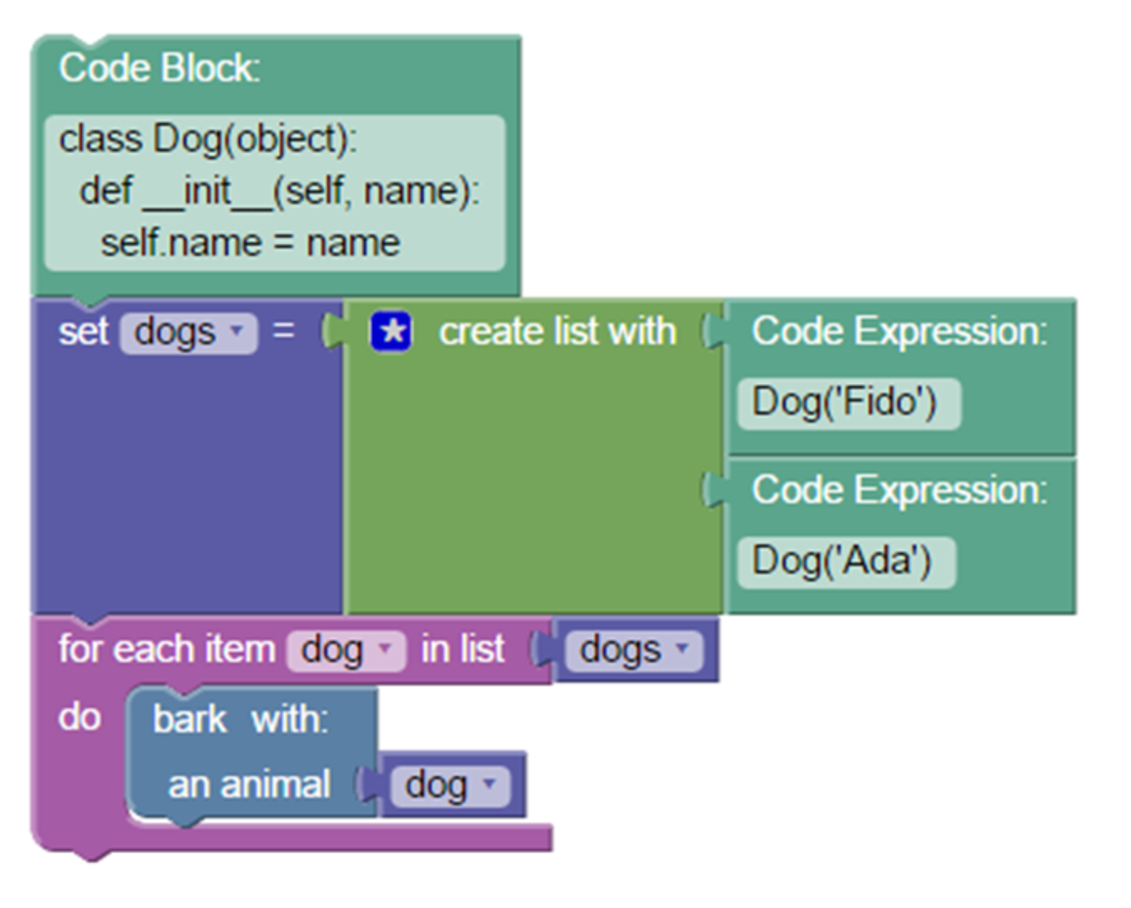
\psfig{file=images/blockly-custom.eps, width=\linewidth}
%\caption{Inline code blocks and expressions provide full support for Python and promotes transfer}
%\label{fig-blockly-custom}
%\end{figure}

We believe that students should perceive authentic value in what they learn, that the material is useful to their long-term goal.
Although some research is working towards creating end-user block-based environments, we view block-based languages as ``Training Wheels'', meant to be faded away.
Work by Weintrop on the transition from Snap to Python analyzes this transition and offers a number of ways to mediate the transfer through programming tools. 
One of the largest findings is that being able to write inline code inside a Block-based language is extremely helpful to students' learning \cite{Weintrop}.
This idea can be pushed further to allow students to convert their block code to textual form and then translate the textual form back to blocks.
This approach, Mutual Language Translation, is also being explored by Matsuzawa\cite{Matsuzawa} to support the transition from a desktop, block-based programming language to Java in an introductory programming class. 
Our environment supports both of these models in order to maximize opportunities to transfer students.
	
	
\section{Questions}

Our new programming environment offers a number of affordances to educators, but much of their promise is still unproven.
Beyond just usability testing, we wish to explore questions relating to the very nature of using data science in a block environment.
One of the major values of a context is being relatable -- it should be a metaphor for students, helping to build on their prior knowledge. Will the entire undergraduate population find data science to be sufficiently relatable? For instance, some students weak math skills or have seriously low self-efficacy with math. Will they find the necessary mathematics (e.g., being able to find the average of a list) too confusing?

Along similar lines, how do we quickly introduce students to a given dataset, and make them comfortable manipulating and understanding the data it contains?
What interaction can the students have with the blocks in order to aid this experience?
In the datasets currently supported by the environment, some are ``easier'' than the others: our students had no trouble working with weather data, for instance, but struggled when confronted by stock trading data.
Are some datasets inherently more suitable for introductory experiences?
And, in general, just how crucial are students' perceptions of interest and usefulness? 

Of course, our environments' affordances also raise more general questions.
In our own experiences with using a block-based environment to scaffold learners into a serious environment, the transfer can be very rocky.
Some students are eager to start using the text-based environment and do not need to pushed to move away from the blocks.
However, some students may be wary about losing their training wheels and, if left to their own devices, may choose to delay trying out the text-based code.
How do we gracefully transition students to writing text, based on the students' ability level, motivational level, and the course's time table?
How does Mutual Language Translation support and hinder this process?

\section{Conclusions}

In this paper, we have introduced our new environment, ``BlockPy'', that promotes Data Science through a block-based interface.
We make a case that by relying on a more generally Useful context, rather than Interest, we can appeal to a wider range of mature learners.
We describe a number of features we seek to support in our environment.
Finally, we discussed the research issues that we are now exploring through this environment.

\bibliographystyle{abbrv}
\bibliography{sigproc}  % sigproc.bib is the name of the Bibliography in this case
% You must have a proper ".bib" file
%  and remember to run:
% latex bibtex latex latex
% to resolve all re


\end{document}